\apendice{Especificación de diseño}

\section{Introducción}
En este apéndice, se recoge la especificación de diseño del proyecto. El objetivo es detallar los aspectos de construcción del sistema, en el que se incluyen:
\begin{itemize}
    \item \textbf{Diseño de datos:} se definen entidades con sus atributos y relaciones entre ellas. También, se definen esquemas de persistencia.
    \item \textbf{Diseño arquitectónico:} se define la estructura interna del sistema, así como la comunicación entre los distintos módulos.
    \item \textbf{Diseño procedimental:} se definen los flujos de interacción entre el cliente y el servicio.
\end{itemize}

\section{Diseño de datos}
En esta sección, se explican los diseños de datos del sistema. A continuación, se explican las entidades que componen el sistema y las relaciones de cada una de ellas.

\subsection{Diccionario de datos}
En este proyecto solo se utiliza una tabla en la base de datos, ya que solo se desea almacenar las tareas personales de un usuario, por lo tanto, solo se requiere la utilización de una tabla. En caso de que existieran más datos a almacenar en la nube, la cantidad de tablas aumentaría.

\begin{figure}[H]
    \centering
    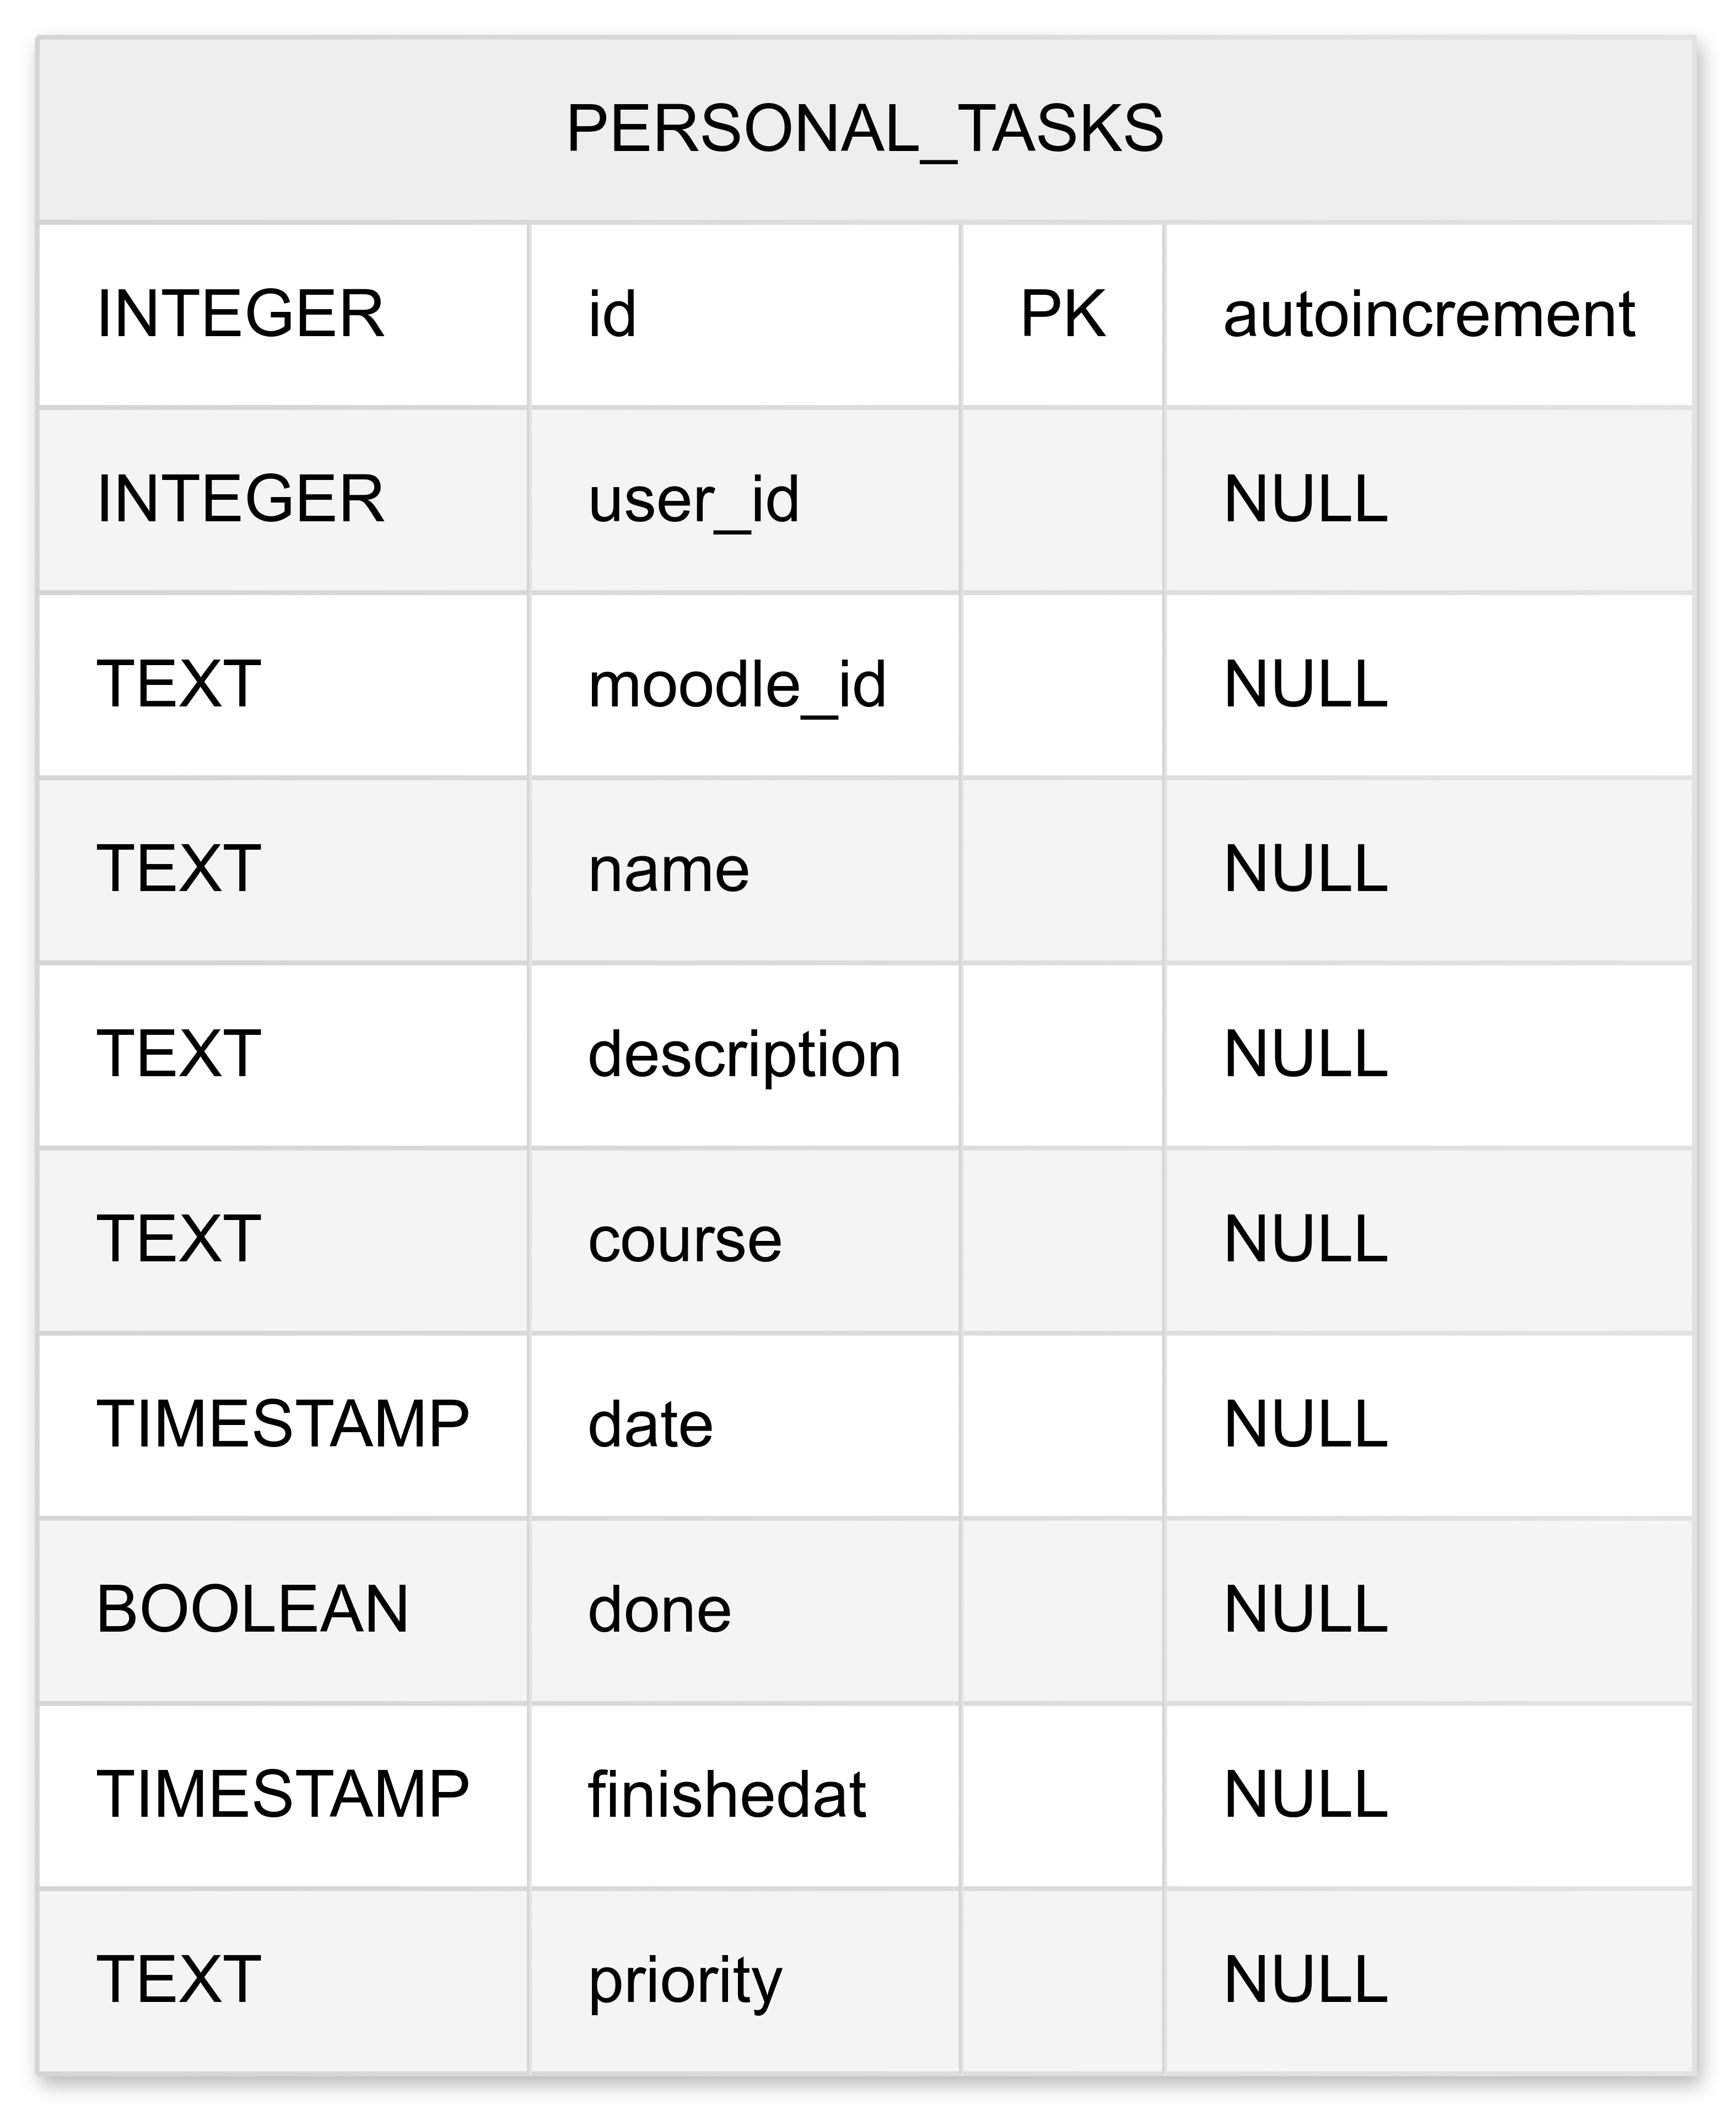
\includegraphics[width=0.6\linewidth]{img/diccionario_datos.png}
    \caption{Diccionario de datos}
    \label{fig:diccionario_datos}
\end{figure}

Se explican los atributos del diccionario de datos anterior:
\begin{itemize}
    \item \textbf{id:} representa el número de identificación de la tarea, es autoincremental Fig. \ref{fig:diccionario_datos}.
    \item \textbf{user\_id:} representa el número de identificación del usuario dentro de la plataforma en la que se encuentre Fig. \ref{fig:diccionario_datos}.
    \item \textbf{moodle\_id:} representa la URL de la plataforma a la que pertenece el usuario Fig. \ref{fig:diccionario_datos}.
    \item \textbf{name:} nombre de la tarea personal Fig. \ref{fig:diccionario_datos}.
    \item \textbf{description:} descripción de la tarea personal Fig. \ref{fig:diccionario_datos}.
    \item \textbf{course:} curso al que pertenece la tarea personal (entre los cursos en los que se encuentra matriculado el usuario propietario de la tarea personal) Fig. \ref{fig:diccionario_datos}.
    \item \textbf{date:} fecha de finalización de la tarea personal Fig. \ref{fig:diccionario_datos}.
    \item \textbf{done:} estado de finalización de la tarea Fig. \ref{fig:diccionario_datos}.
    \item \textbf{finishedat:} fecha en la que se finaliza la tarea Fig. \ref{fig:diccionario_datos}.
    \item \textbf{priority:} prioridad de la tarea Fig. \ref{fig:diccionario_datos}.
\end{itemize}

\subsection{Modelos de datos}
A continuación, se muestra un diagrama de clases para comprender la relación entre los distintos modelos de datos de la aplicación y la función de cada uno de ellos.

\begin{figure}[H]
    \centering
    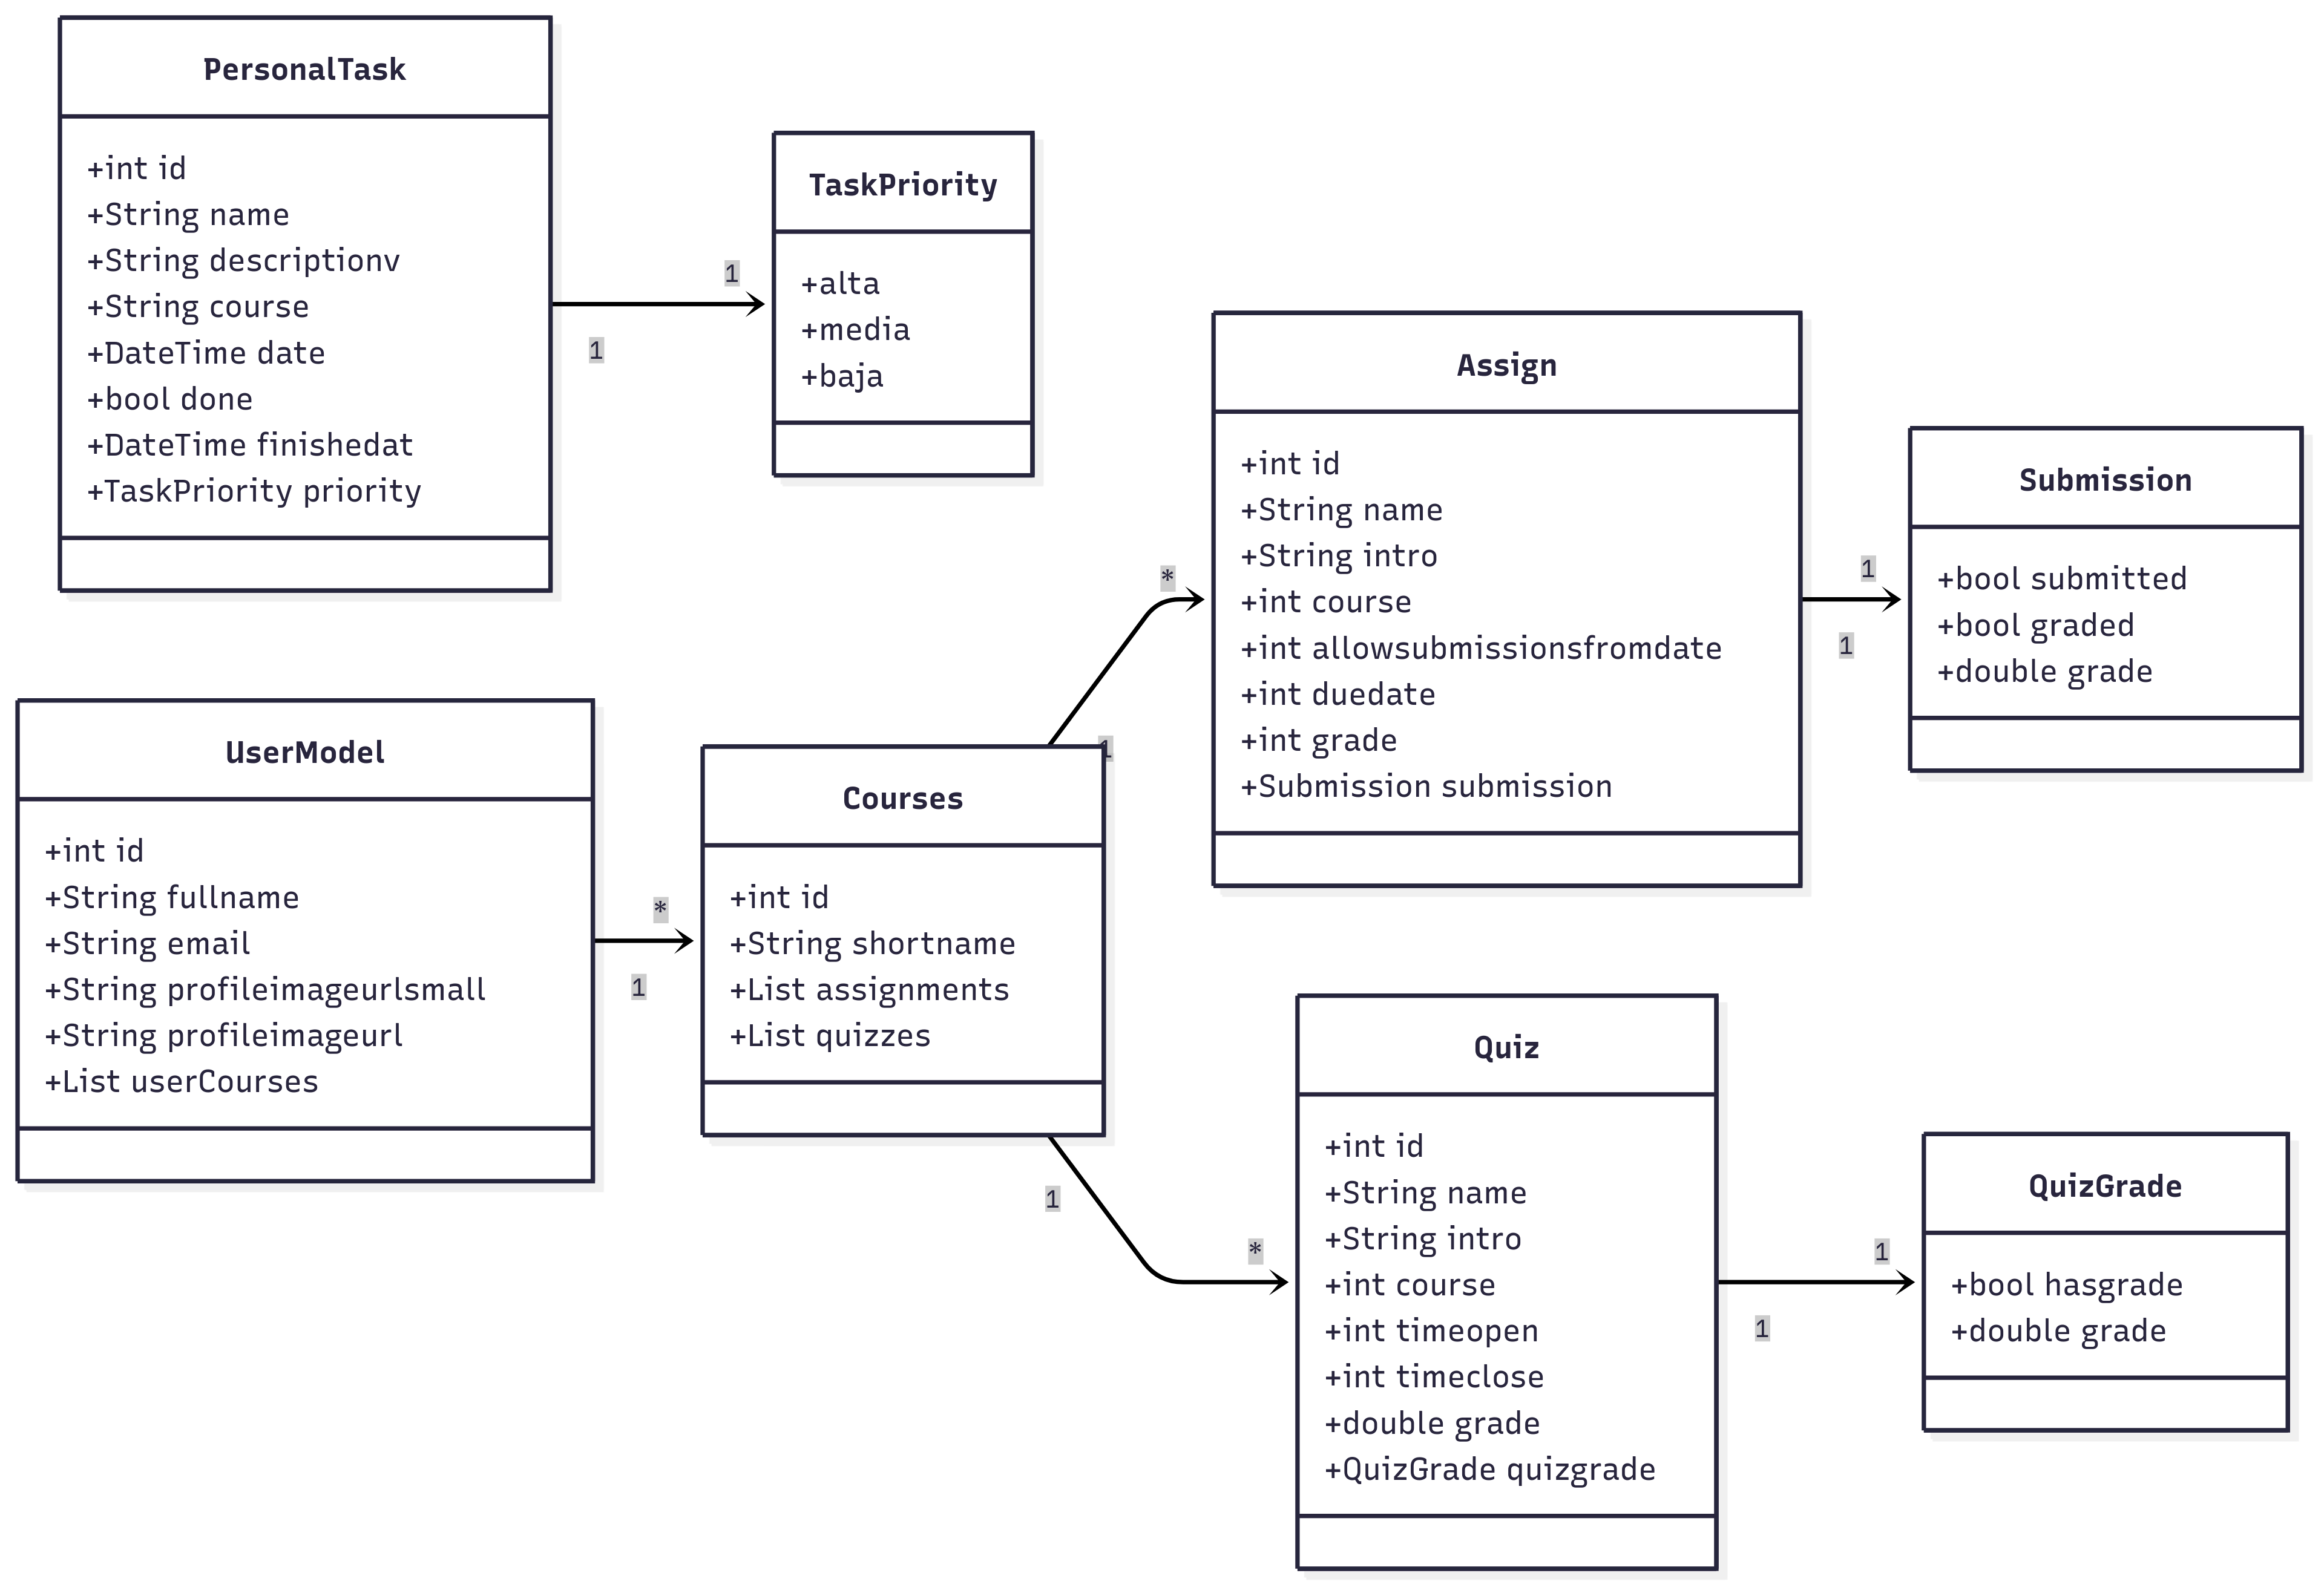
\includegraphics[width=1.0\linewidth]{img/modelo_datos.png}
    \caption{Diagrama de Modelo de datos}
    \label{fig:modelo_datos}
\end{figure}

En los modelos hay definidos más atributos, pero en el diagrama \ref{fig:modelo_datos} se representan aquellos que han sido empleados en el proyecto. A continuación se detalla cada uno de ellos:
\tablaSmallSinColores
{Modelo UserModel}
{lcc}
{modelo-usermodel}
{
    \textbf{Atributo} & \textbf{Tipo} & \textbf{Contenido} \\
}
{
    id & int & Número de identificación del usuario.\\
    fullname & String & Nombre completo del usuario.\\
    email & String & Correo electrónico del usuario.\\
    profileimageurlsmall & String & Dirección de imágen de perfil del usuario.\\
    profileimageurl & String & Dirección de imágen de perfil del usuario.\\
    userCourses & Lista & Lista de cursos del usuario.\\
}

\tablaSmallSinColores
{Modelo Courses}
{lcc}
{modelo-courses}
{
    \textbf{Atributo} & \textbf{Tipo} & \textbf{Contenido} \\
}
{
    id & int & Número de identificación del curso.\\
    shortname & String & Nombre corto del curso.\\
    assingments & Lista(Assign) & Lista de tareas del curso.\\
    quizzes & Lista(Quiz) & Lista de cuestionarios del curso.\\
}

\tablaSmallSinColores
{Modelo Assign}
{lcp{6cm}}
{modelo-assign}
{
    \textbf{Atributo} & \textbf{Tipo} & \textbf{Contenido} \\
}
{
    id & int & Número de identificación de la tarea.\\
    name & String & Nombre de la tarea.\\
    intro & String & Descripción de la tarea.\\
    course & int & Número de identificación del 
                    curso de la tarea.\\
    allowsubmissionsfromdate & int & Fecha de apertura de la tarea.\\
    duedate & int & Fecha de cierre de la tarea.\\
    grade & int & Tipo de calificación.\\
    submission & Submission & Entrega de la tarea.\\
}

\tablaSmallSinColores
{Modelo Quiz}
{lcc}
{modelo-quiz}
{
    \textbf{Atributo} & \textbf{Tipo} & \textbf{Contenido} \\
}
{
    id & int & Número de identificación del cuestionario.\\
    name & String & Nombre del cuestionario.\\
    intro & String & Descripción del cuestionario.\\
    course & int & Número de identificación del curso del cuestionario.\\
    timeopen & int & Fecha de apertura del cuestionario.\\
    timeclose & int & Fecha de cierre del cuestionario.\\
    grade & double & Tipo de calificación.\\
    quizgrade & QuizGrade & Entrega del cuestionario.\\
}

\tablaSmallSinColores
{Modelo Submission}
{lcc}
{modelo-submission}
{
    \textbf{Atributo} & \textbf{Tipo} & \textbf{Contenido} \\
}
{
    submitted & bool & Estado de entrega de la tarea.\\
    graded & bool & Estado de calificación de la entrega.\\
    grade & double & Calificación de la entrega.\\
}

\tablaSmallSinColores
{Modelo QuizGrade}
{lcc}
{modelo-quizgrade}
{
    \textbf{Atributo} & \textbf{Tipo} & \textbf{Contenido} \\
}
{
    hasgrade & bool & Estado de calificación del cuestionario.\\
    grade & double & Calificación del cuestionario.\\
}

\tablaSmallSinColores
{Modelo PersonalTask}
{lcc}
{modelo-pesonaltask}
{
    \textbf{Atributo} & \textbf{Tipo} & \textbf{Contenido} \\
}
{
    id & int & Número de identificación dela tarea personal.\\
    name & String & Nombre de la tarea personal.\\
    description & String & Descripción de la tarea personal.\\
    course & String & Nombre del curso de la tarea personal.\\
    date & DateTime & Fecha de cierre de la tarea personal.\\
    done & bool & Estado de finalización de la tarea personal.\\
    finishedat & DateTime & Fecha de finalización de la tarea personal.\\
    priority & TaskPriority & Tipo de prioridad de la tarea personal.\\
}

\tablaSmallSinColores
{Modelo TaskPriority}
{lc}
{modelo-taskpriority}
{
    \textbf{Atributo} & \textbf{Contenido} \\
}
{
    alta & Prioridad alta.\\
    baja & Prioridad media.\\
    media & Prioridad baja.\\
}

\section{Diseño arquitectónico}
El diseño arquitectónico empleado en PlanLMS se basa en una estructura modular, que persigue lograr una organización clara de las funcionalidades y responsabilidades, con el fin de garantizar la facilidad en el mantenimiento y escalabilidad del proyecto.

\begin{figure}[H]
    \centering
    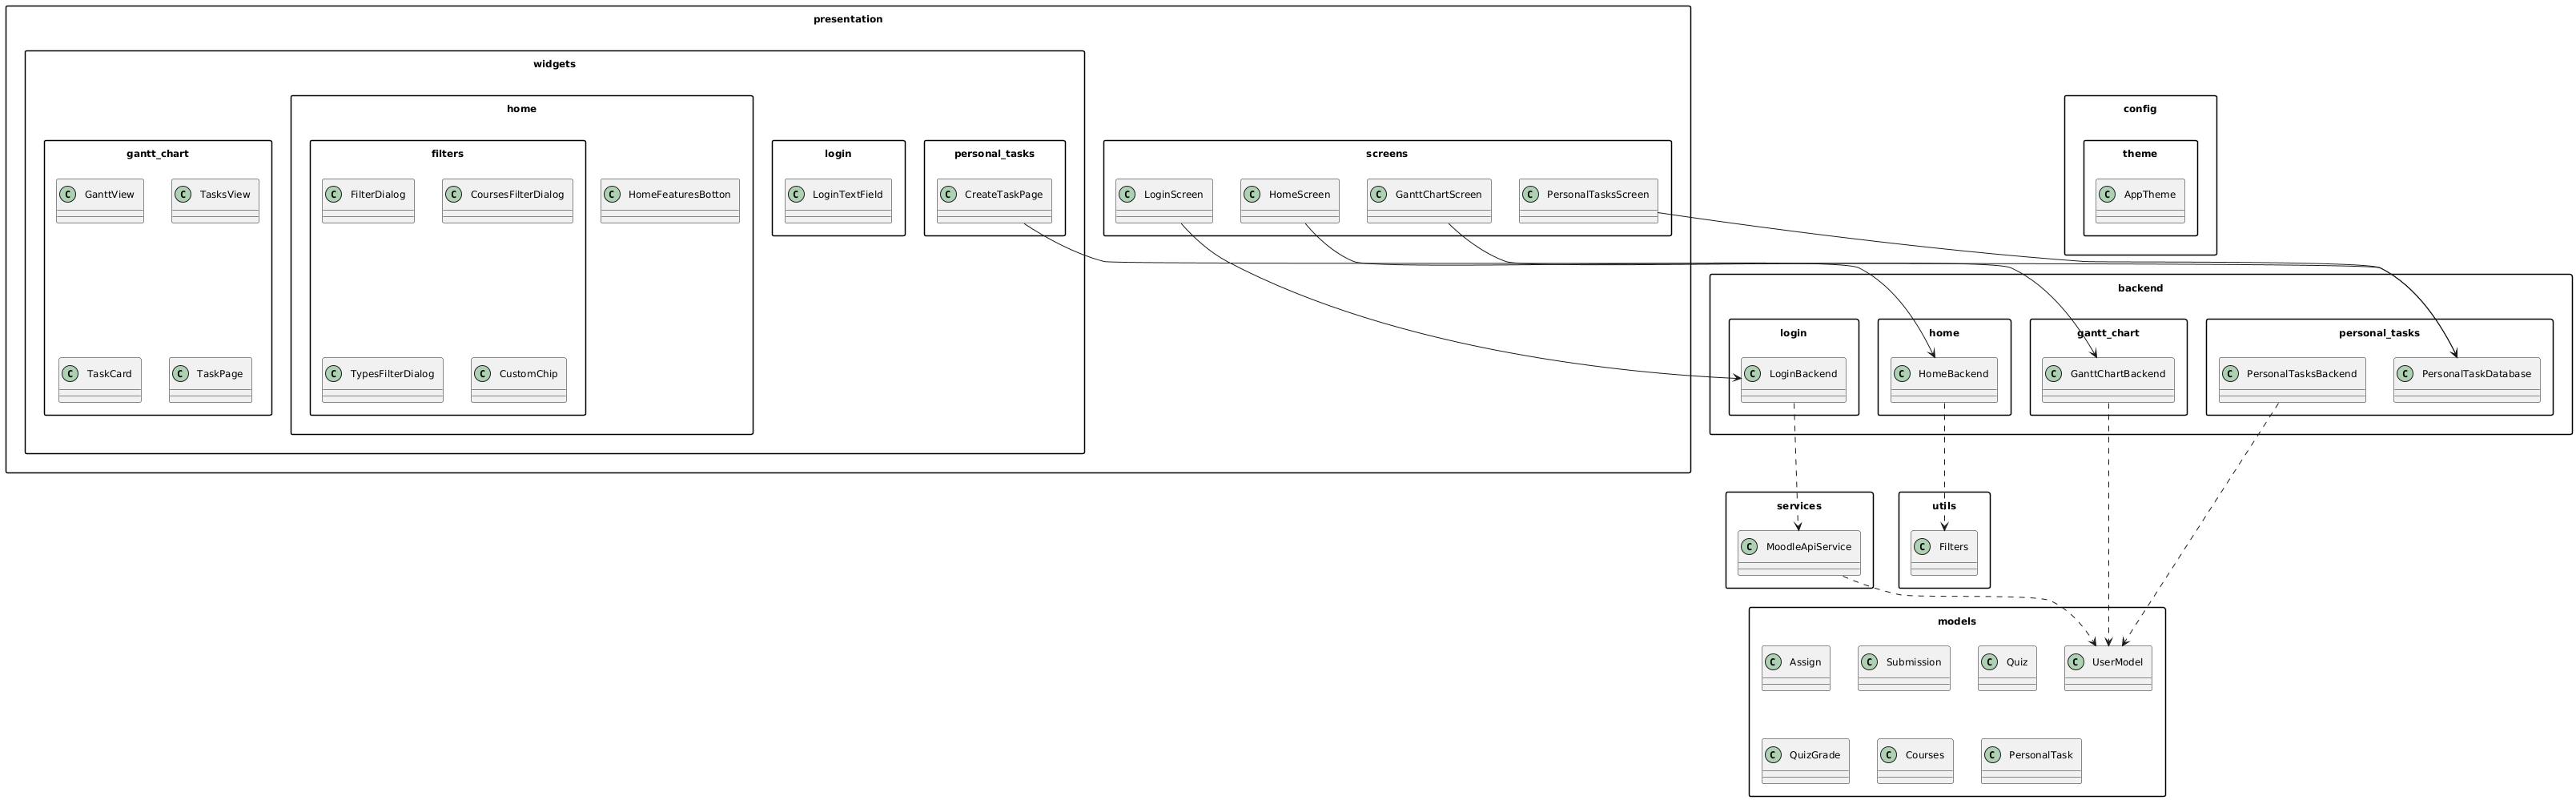
\includegraphics[width=1.3\linewidth]{img/diagrama_clases.png}
    \caption{Diseño arquitectónico del proyecto}
    \label{fig:diagrama_clases}
\end{figure}

A continuación, se detallan los objetivos de cada responsabilidad y funcionalidad:
\begin{itemize}
    \item \textbf{presentation:} contiene todos los elementos de interfaz gráfica Fig. \ref{fig:diagrama_clases}. Este paquete se divide en dos paquetes:
        \begin{itemize}
            \item \textbf{screens:} contiene las pantallas de la aplicación.
            \item \textbf{widgets:} contiene algunos widgets que componen las pantallas, con el fin de aprovechar la reutilización de estos.
        \end{itemize}
        Estos dos paquetes se dividen en otros más pequeños, cada uno asociado a una funcionalidad de la aplicación.
    \item \textbf{config:} contiene elementos de configuración de temas estéticos de algun componente Fig. \ref{fig:diagrama_clases}.
    \item \textbf{backend:} contiene la lógica de negocio, se encarga de gestionar los datos de cada capa de presentación Fig. \ref{fig:diagrama_clases}.
    \item \textbf{services:} se encarga de la comunicación con lo servicios externos Fig. \ref{fig:diagrama_clases}.
    \item \textbf{utils:} contiene los elementos que son empleados por las diferentes clases de la arquitectura Fig. \ref{fig:diagrama_clases}.
    \item \textbf{models:} contiene todas las entidades y define las estructuras de estas Fig. \ref{fig:diagrama_clases}.
\end{itemize}

\subsection{Estrategias de persistencia}
La persistencia de los datos dentro del sistema, se reparte en tres formas:
\begin{itemize}
    \item \textbf{SharedPreferences:} se encarga de almacenar los filtros de los usuarios para poder restaurarlos cada vez que se inicia la aplicación. Además, también guarda el correo electrónico de inicio de sesión.
    \item \textbf{Supabase:} se encarga de almacenar las tareas personales de todos los usuarios. Cada vez que se consulta Supabase se retorna la lista más reciente de tareas del usuario.
    \item \textbf{Caché en memoria:} se encarga de almacenar los datos de la sesión del usuario. Algunos de estos datos son los cursos, tareas, cuestionarios, entregas, calificaciones, etc.
\end{itemize}

\subsection{Seguridad}
En el directorio del proyecto existe un archivo denominado \textit{.env}, que alberga las claves para acceder a la base de datos de Supabase. Estos ficheros se excluyen de la sincronización del repositorio en la nube. Evitando que cualquier usuario no deseado pudiera acceder a los datos.

Por otra parte, el \textit{token} privado que proporciona el \textit{Web Service de Moodle} se mantiene en memoria, además, de que al cerrar sesión este se elimina de memoria.

Por último, todas las peticiones HTTP van por HTTPS, lo que quiere decir, que todas las peticiones emplean un protocolo de comunicación seguro donde los datos no van a ser leídos por terceros.

\section{Diseño procedimental}
A continuación, se muestran diagramas de secuencia que representan el funcionamiento interno de la aplicación.

\subsection{Inicio de sesión}
La Figura \ref{fig:secuencia_login} describe el comportamiento del sistema cuando el usuario inicia sesión en PlanLMS.

\begin{enumerate}
    \item El usuario introduce el correo electrónico y contraseña y presiona el botón "Iniciar sesión".
    \item \textbf{LoginScreen} le pide a su \textit{backend} que ejecute \textbf{loginSetup(email, pass, saveEmail)}, que a su vez, solicita a \textbf{MoodleAPIService} que ejecute \textbf{login(username, password)}.
    \item Una vez obtenido el \textit{token}, se almacena opcionalmente el email con \textbf{SharedPreferences}, y solicita los datos del usuario y sus cursos a \textbf{MoodleAPIService}, mediante \textbf{getUserInfo()} y \textbf{getUserCourses(userId)}.
    \item Realiza iteraciones para cada curso, obteniendo las tareas (\textbf{getCourseAssignments()}) y cuestionarios (\textbf{getCourseQuizzes()}) de cada uno, así como los estados de entrega de cada una de las actividades (\textbf{getAssignSubmissionStatus()} y \textbf{getQuizSubmissionStatus()}).
    \item Toda la información extraída, se convierte en objetos que se asignan al \textbf{UserModel} y a \textbf{Course},posteriormente se retorna a \textbf{LoginScreen} y se navega al \textbf{HomeScreen}.
\end{enumerate}

\begin{figure}[p]
    \centering
    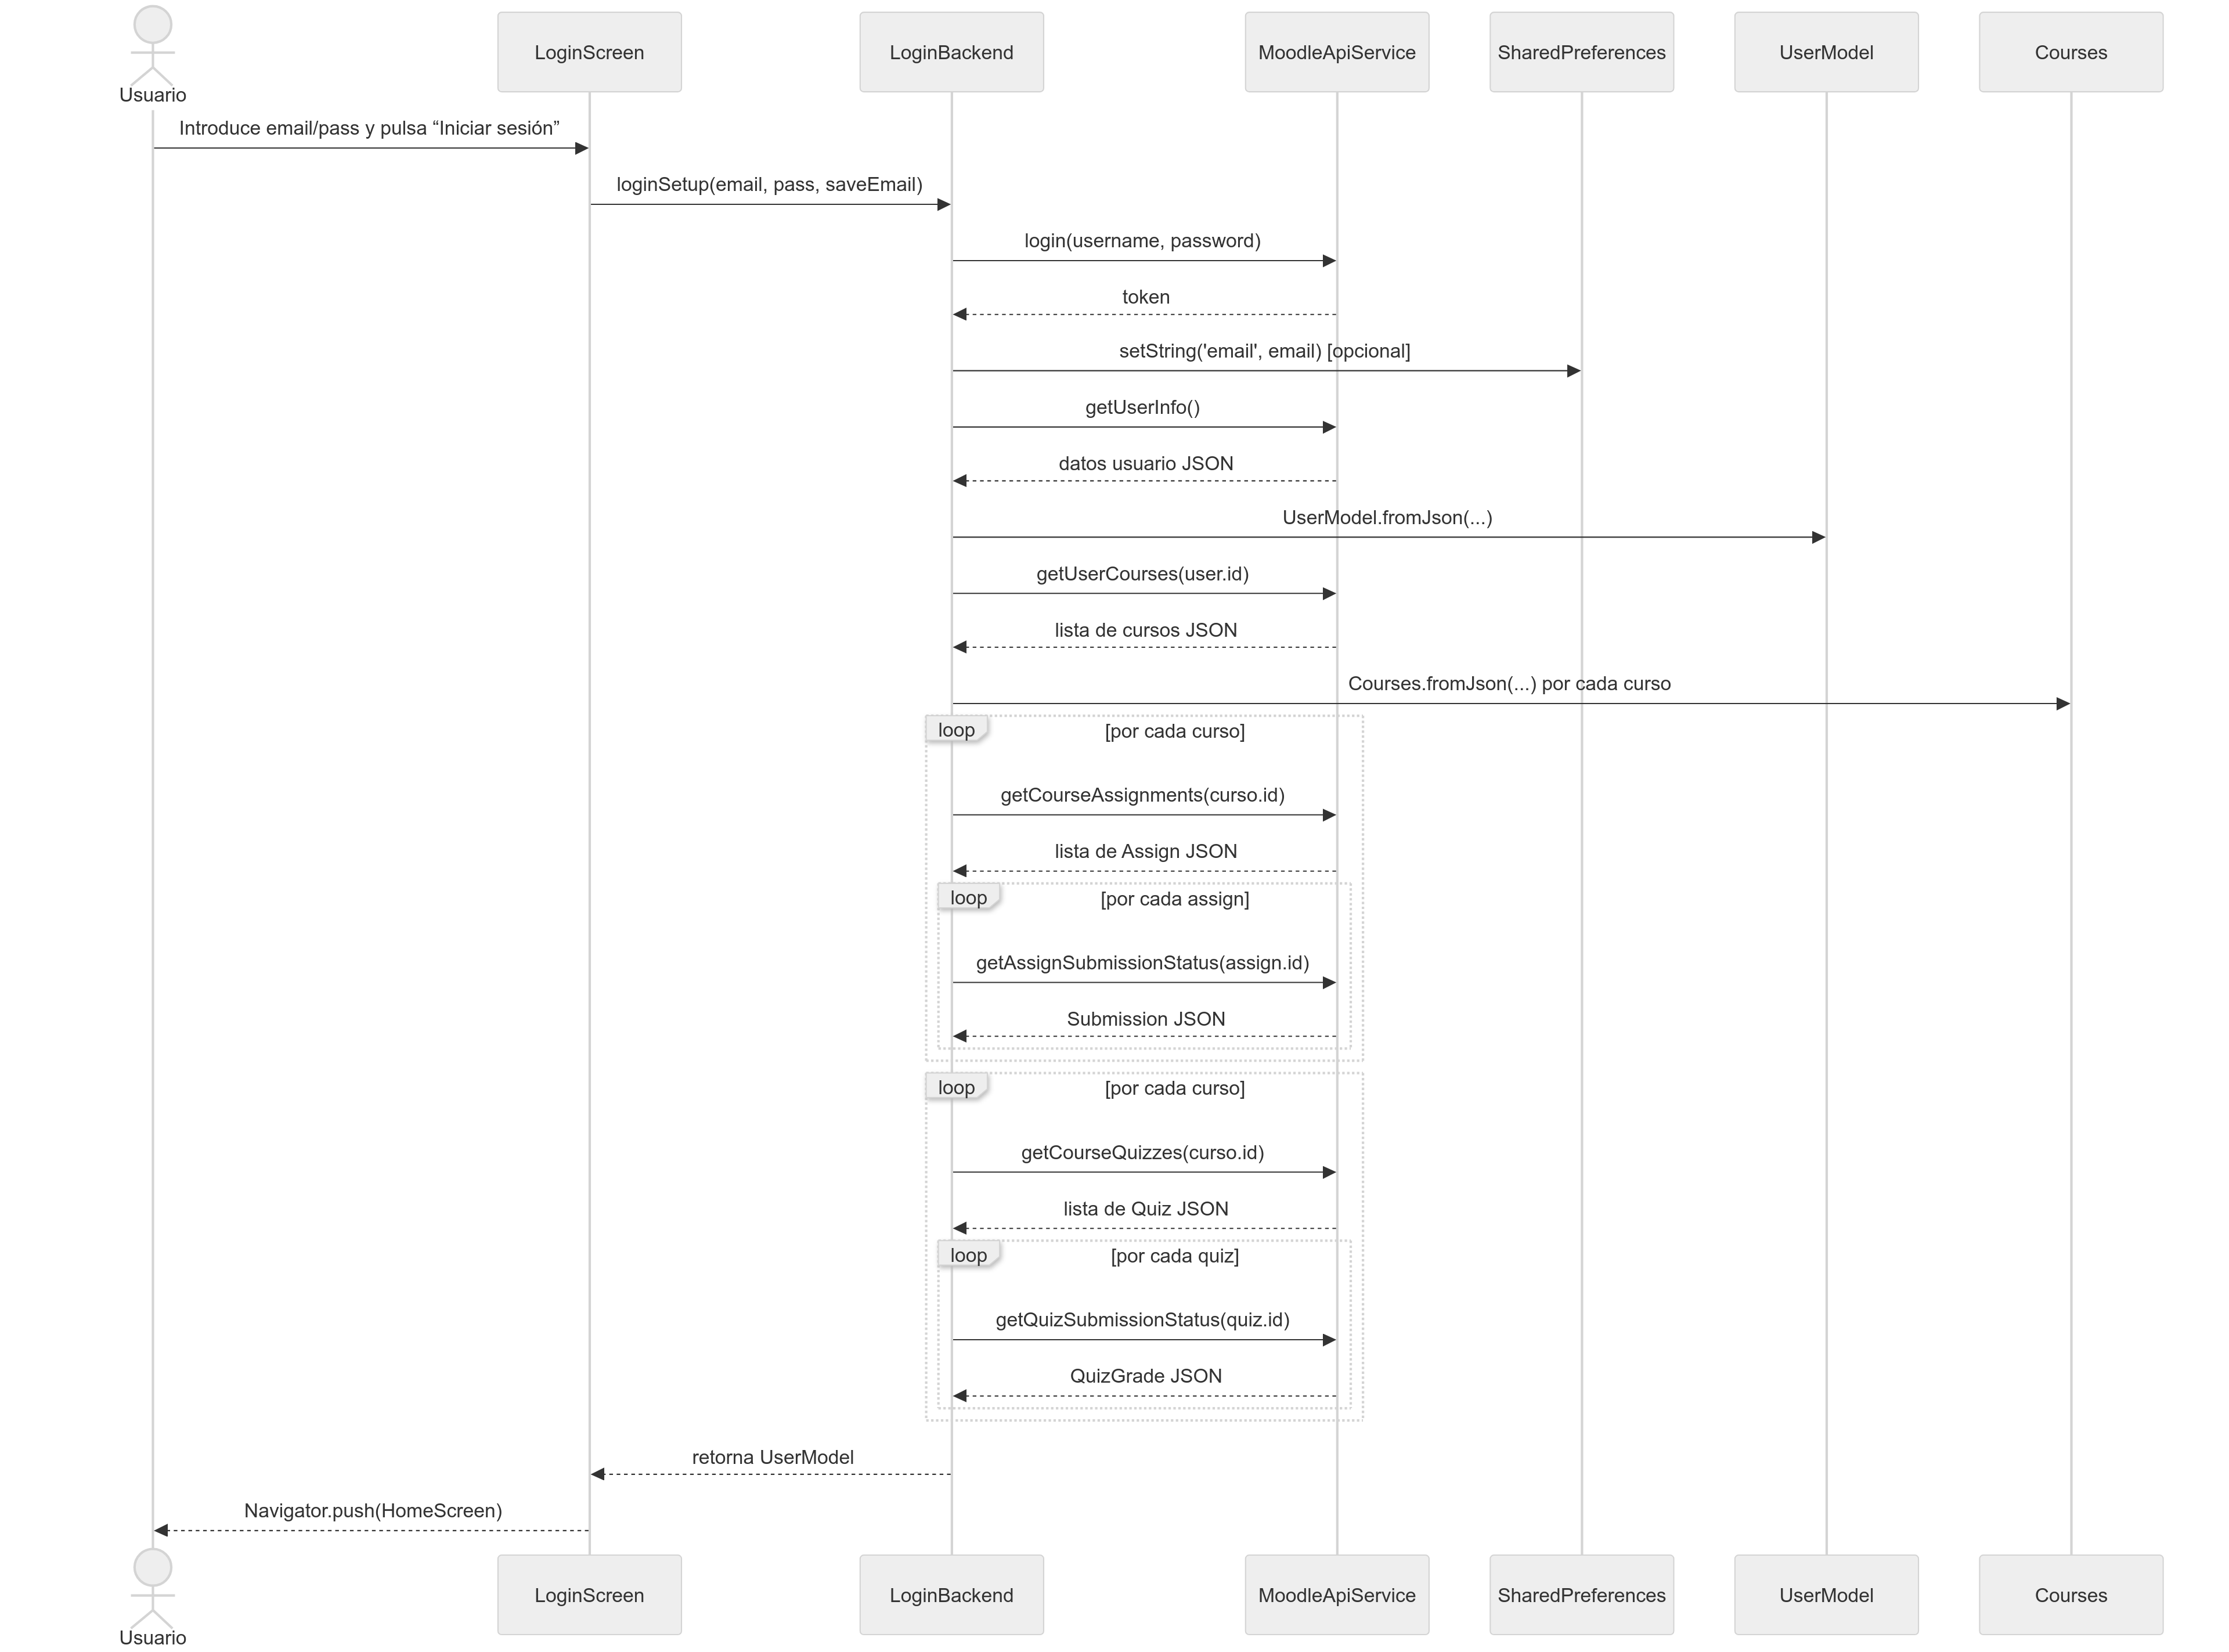
\includegraphics[width=1.2\linewidth]{img/secuencia_login.png}
    \caption{Diagrama de secuencia del inicio de sesión}
    \label{fig:secuencia_login}
\end{figure}

\subsection{Creación de tareas personales}
La Figura \ref{fig:secuencia_creacion_tareas} describe el comportamiento del sistema cuando el usuario procede con la creación de una tarea personal.

\begin{enumerate}
    \item El usuario abre el formulario y lo rellena. Al pulsar el botón \textit{Guardar} se realiza una llamada a \textbf{validateFields()} que se encarga de verificar que todos los campos del formulario han sido rellenados.
    \item Si la verificación es correcta, se ejecuta \textbf{createPersonalTask(PersonalTask)} de PersonalTaskDatabase, para realizar la inserción de la nueva tarea en la base de datos en la nube.
    \item Cuando se confirma la inserción, se realiza una llamada a \textbf{widget.refreshTasks()} que hace referencia a \textbf{loadTasks()} de \textbf{PersonalTasksScreen}, se actuliza la lista de tareas y se muestra la nueva tarea.
    \item En caso de que no se rellene el formulario con los datos necesarios, se muestra un \textbf{SnackBar} indicando \textit{Rellene los campos}.
\end{enumerate}

\begin{figure}[p]
    \centering
    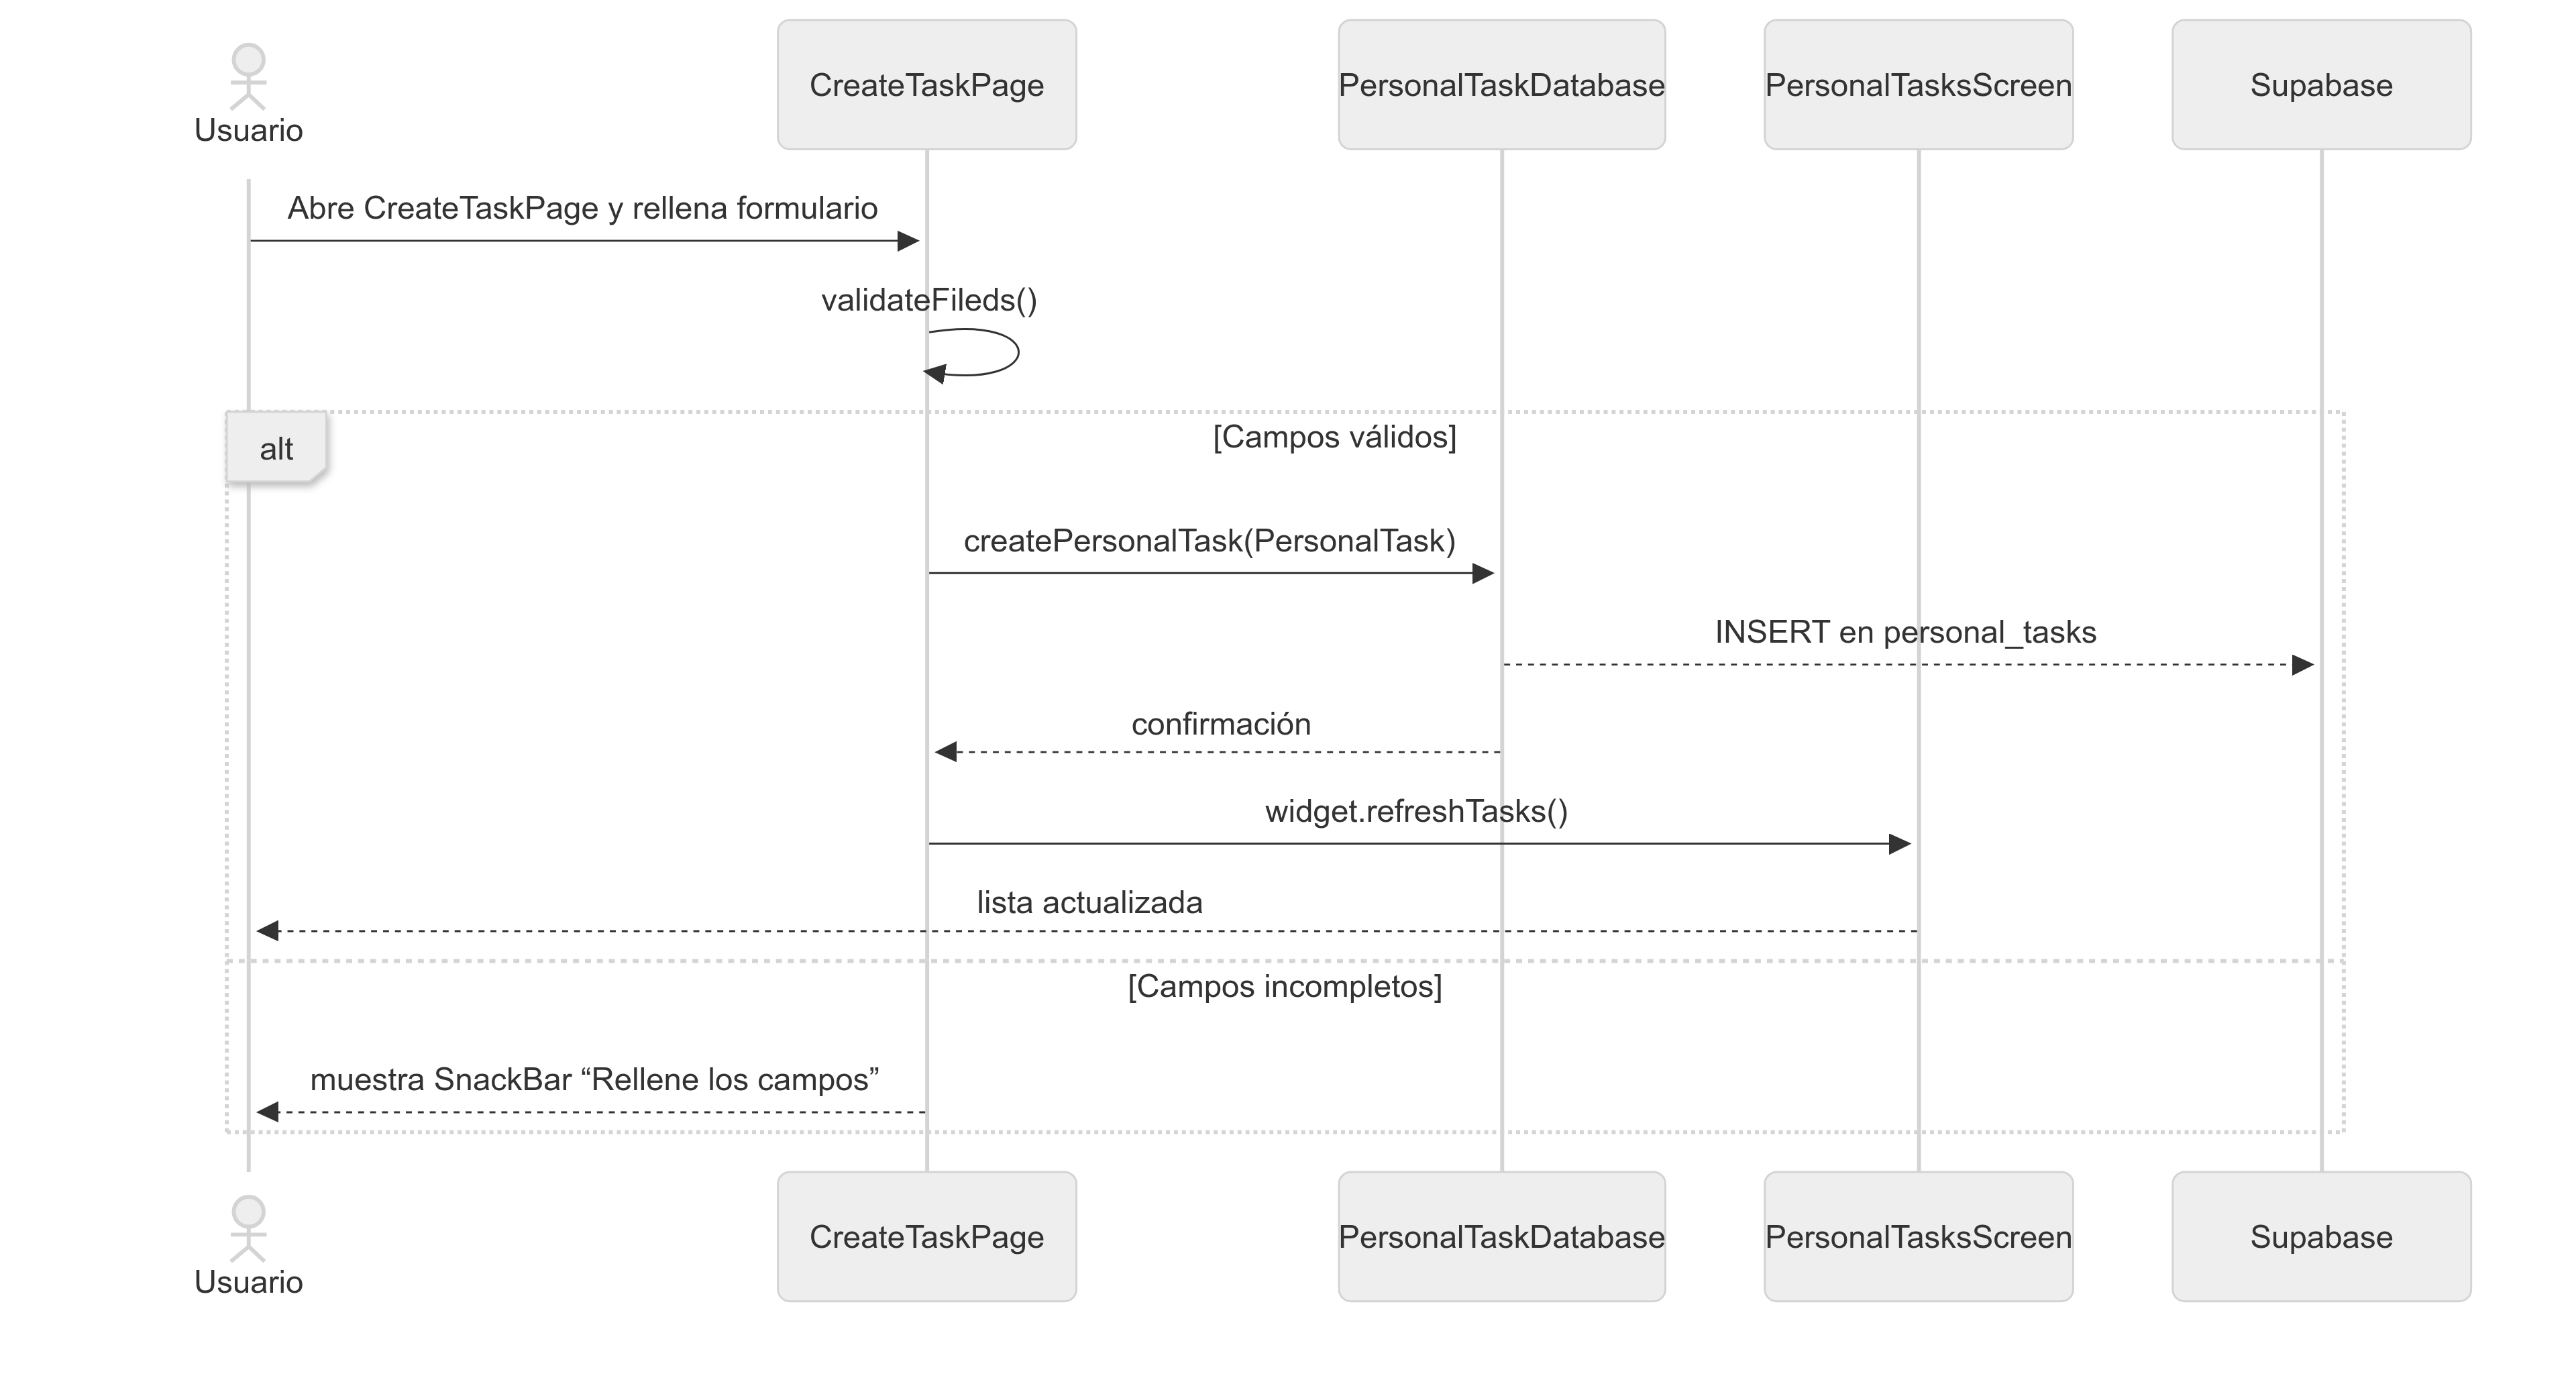
\includegraphics[width=1.0\linewidth]{img/secuencia_creacion_tareas.png}
    \caption{Diagrama de secuencia de la creación de tareas}
    \label{fig:secuencia_creacion_tareas}
\end{figure}

\subsection{Eliminación de tareas personales}
La Figura \ref{fig:secuencia_eliminar_tarea} describe el comportamiento del sistema cuando el usuario procede con la eliminación de una tarea personal.

\begin{enumerate}
    \item El usuario desliza la tarjeta de la tarea y pulsa en el icono de \textit{Eliminar}.
    \item \textbf{TaskCard} llama a la función \textbf{deleteTask(task)} de \textbf{PersonalTaskDatabase}, que solicita la base de datos eliminar la tarea personal de la tabla \textit{personal\_tasks}.
    \item Tras confirmar que se ha eliminado correctamente, se retorna de nuevo a \textbf{TaskCard}, que lanza la orden de ejecutar \textbf{refereshTasks()}, que repite el mismo proceso que la Figura \ref{fig:secuencia_creacion_tareas}.
\end{enumerate}

\begin{figure}[p]
    \centering
    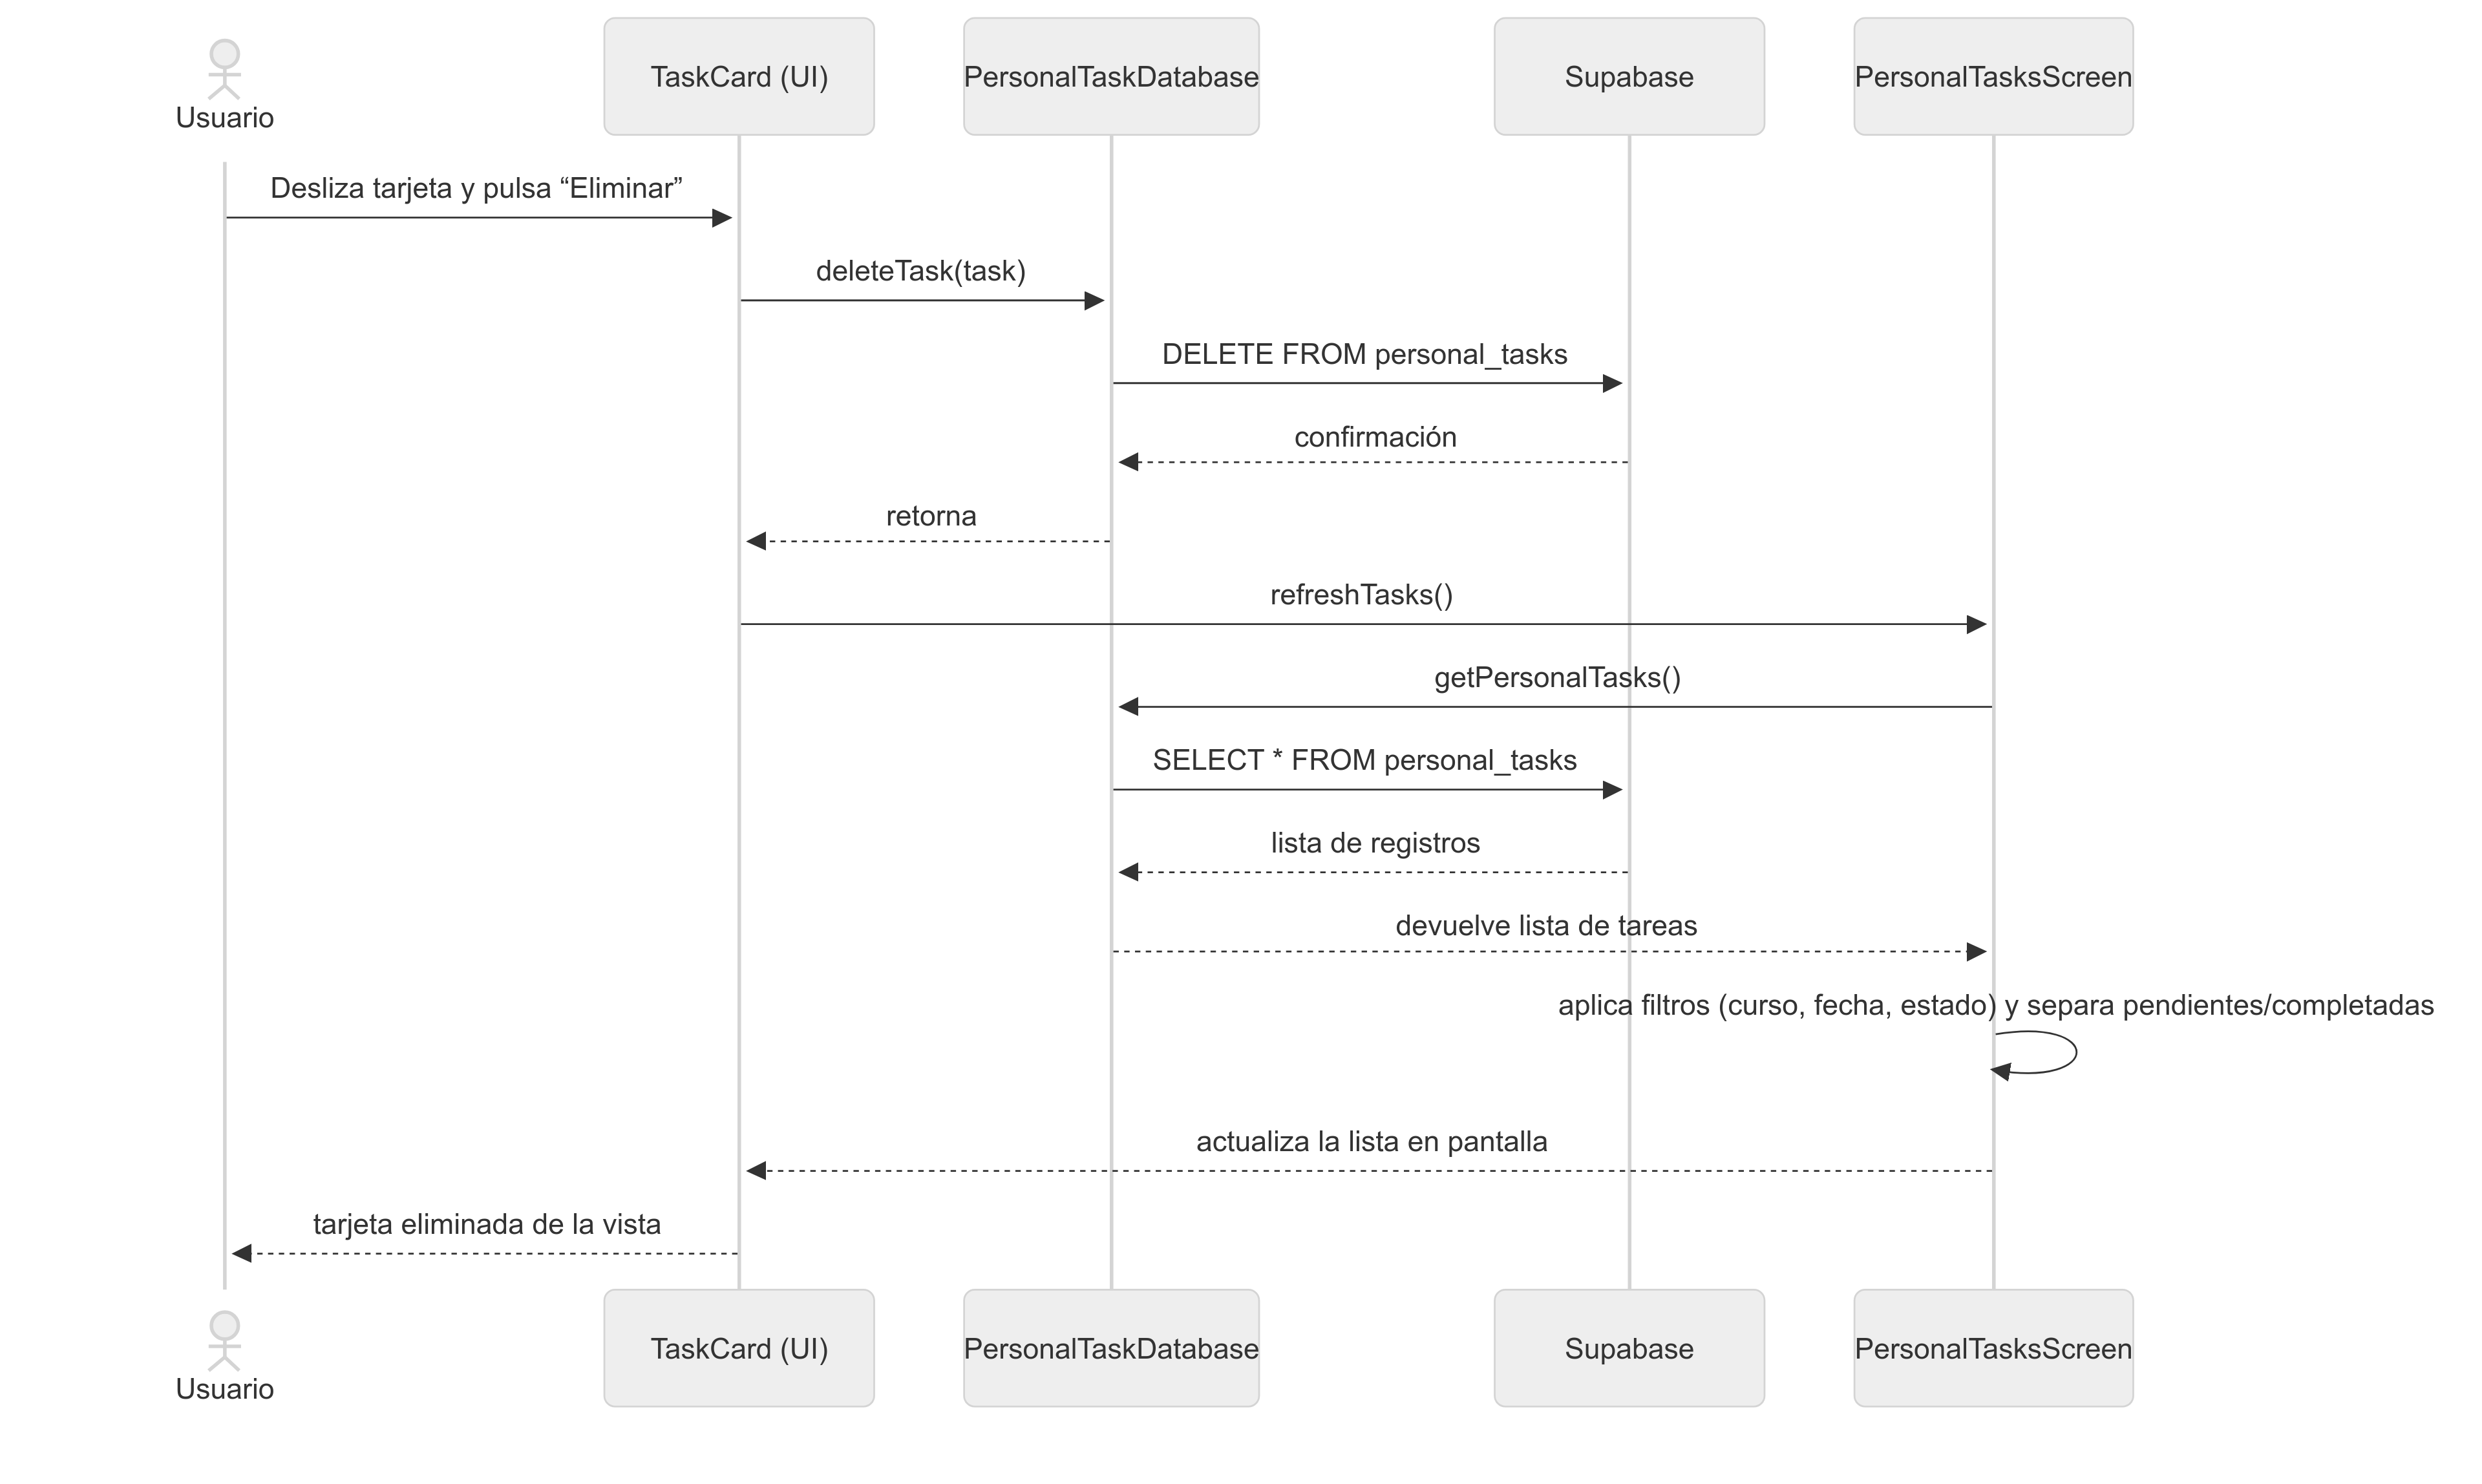
\includegraphics[width=1.0\linewidth]{img/secuencia_eliminar_tarea.png}
    \caption{Diagrama de secuencia de la eliminación de tareas}
    \label{fig:secuencia_eliminar_tarea}
\end{figure}